% !TeX spellcheck = ru_RU
\documentclass{article}

\usepackage{amsthm}
\usepackage{amssymb}
\usepackage{amsmath}
\usepackage{enumitem}
\usepackage{graphicx}
\usepackage{float}
\usepackage[a4paper, total={6in, 10in}]{geometry}
\usepackage{algorithm}
\usepackage{algpseudocode}
\usepackage{hyperref}


\usepackage[T2A]{fontenc}
\usepackage[utf8]{inputenc}
\usepackage[russian]{babel}
\usepackage{yfonts}

% \usepackage[
% backend=biber,
% style=alphabetic,
% sorting=ynt
% ]{biblatex}
% \addbibresource{ref.bib}

% \DeclareMathOperator{\deg}{deg}

\newtheorem{definition}{Определение}
\newtheorem{lemma}{Лемма}
\newtheorem{theorem}{Теорема}
\newtheorem{task}{Задача}
\newtheorem{corollary}{Следствие}

\newenvironment{solution}{\textit{Решение:}}{\hfill$\square$}

\newtheoremstyle{break}
{\topsep}{\topsep}%
{\itshape}{}%
{\bfseries}{}%
{\newline}{}%
\theoremstyle{definition}


\title{Взвешенная задача вершинного покрытия и алгоритмы аппроксимации}
\author{Бруёк Алексей, Б05-022}
\date{}

\begin{document}
	\maketitle
  \begin{abstract}
    В этой работе описан жадный алгоритм $2$-приближения минимального вершинного покрытия
    с доказательством коррестности и результатами тестирования. 
    Основным источником стала книга \cite{main_source}.
  \end{abstract}
  \section{Упрощенные постановки задачи}
  \subsection{Невзвешенный случай}
  \begin{definition}
    \text{Минимальным вершинным покрытием} называется наименьшее 
    по мощности подмножество вершин графа, являющееся вершинным покрытием графа.
  \end{definition}
  \begin{task}
    Найти вершинное покрытие, мощности не более чем в 2 раза большей, 
    чем у минимального за полиномиальное время. (Полиномиальный алгоритм 2-приближения)
  \end{task}
  Очевидно, что найдя максимальное по включению паросочетание, 
  мы сможем выбрать вершины, входящие в это паросочетание и получить вершинное покрытие.
  При этом минимальное вершинное покрытие должно содержать по крайне мере по одной вершине
  из каждого из этих ребер, поэтому мы не ухудшим ответ более чем в 2 раза.
  \subsection{Функция весов пропорциональна $deg$}
  \begin{definition}
    Назовем функцию весов $w: V \rightarrow \mathbb{Q}^+$ пропорционально-степенной,
    если существует такая константа $c \in \mathbb{Q}^+$, что
    $$\forall v \in V: w(v) = c \cdot deg(v)$$
    где $deg(v)$ -- степень вершины $v$.
  \end{definition}
  \begin{definition}
    Минимальным вершинным покрытием во взвешенном случае называем вершинное покрытие минимального веса.
  \end{definition}
  \begin{task}
    Дан граф $G$ с пропорционально-степенной функцией весов $w$, нужно найти
    2-приближение минимального вершинного покрытия за полиномиальное время.
  \end{task}
  \begin{lemma}
    Если $w$ пропорционально-степенная функция весов и $OPT$ -- минимальное вершинное покрытие,
    то 
    $$w(V) \le 2\cdot w(OPT)$$
  \end{lemma}
  \begin{proof}
    $$w(V) = \sum_{v\in V}c\cdot deg(v) = c \sum_{v \in V} deg(v) = 2c|E|$$
    $$w(OPT) = \sum_{v \in OPT}c\cdot deg(v) = c \sum_{v \in OPT}deg(v)$$
    Так как для каждого ребра, хотя бы один из его концов принадлежит $OPT$,
    имеем 
    $$\sum_{v \in OPT} deg(v) \ge |E|$$
    В итоге,
    $$2w(OPT) \ge 2c|E| = w(V)$$
  \end{proof}
  \begin{corollary}\label{corollarySimpleWeight}
    В случае пропорционально степенной функции весов, веса любых 2-x вершинных покрытий
    отличаются не более чем в 2 раза.
  \end{corollary}
  \section{Основная задача}
  \begin{task}
    Дан граф $G$ и произвольная функция весов $w$. 
    Требуется найти 2-приближение минимального вершинного покрытия за полиномиальное время.
  \end{task}
  \begin{algorithm}[H]
    \caption{GreedyAlgo}\label{greedyAlgo}
    \begin{algorithmic}
      \Require $G = (V, E)$, $w:V \rightarrow \mathbb{Q}^+$ -- функция весов
      \State $S \gets \emptyset$ -- итоговое вершинное покрытие
      \While{$V \ne \emptyset$}
        \State $c \gets \min_{v \in V}\frac{w(v)}{deg(v)}$
        \State $t(v) \gets c\cdot deg(v)$ --         
        \State $w \gets w - t$
        \State $D \gets \{v\in V: w(v) = 0\}$
        \State $S \gets S \cup D$ -- добавляем вершины в ответ
        \State $V \gets V \backslash D$ -- и удаляем их из графа
        \State $V \gets V \backslash \{v \in V: deg(v) = 0\}$ 
      \EndWhile\\
      \Return{$S$}
    \end{algorithmic}
  \end{algorithm}

  \textbf{Краткое описание алгоритма:}
  На каждой итерации:
  \begin{itemize}
    \item находим максимальную пропорционально-степенную 
  функцию весов $t$, которая не превосходит $w$ на всех вершинах и вычитаем ее из $w$.
    \item Вершины вес которых стал нулевым добавляем в ответ и удаляем из графа.
    \item Вершины с нулевымы степенями просто удаляем
  \end{itemize}
  Очевидно, алгоритм удаляет вершины на каждом шаге, а значит он закончится и вернет ответ $S$.\\
  Убедимся в корретности ответа
  \begin{lemma}
    Множество вершин $S$ полученное алгоритмом (\ref{greedyAlgo}) 
    является вершинным покрытием.
  \end{lemma}
  \begin{proof}
    Пусть $(u, v) \in E$ и вершины $u$, $v$ не вошли в $S$.\\
    Тогда $u$, $v$ должны были быть удалены как вершины с нулевой степенью, 
    что невозможно.
  \end{proof}
  Теперь докажем, что \ref{greedyAlgo} является алгоритмом 2-приближения.\\
  Введем обозначения:
  \begin{itemize}
    \item $t_i$ -- пропорционально-степенная функция весов, полученная на $i$-ой итерации
    \item $G_i=(V_i, E_i)$ -- граф перед $i$-ой итерацией.
    \item $S$ -- ответ алгоритма
    \item $OPT$ -- настоящее минимальное вершинное покрытие
    \item $k$ -- количество итераций алгоритма
    \item $w$ -- исходная функция весов
  \end{itemize}
  \begin{lemma}\label{greedySumElementLem}
    $$
      \forall i \in \mathbb{N} \cap \left[1, k\right]
      \forall j \in \mathbb{N} \cap \left[j, k\right]: 
      t_i(G_j \cap S) \le 2t_i(G_j \cap OPT)
    $$
  \end{lemma}
  \begin{proof}
    Зафикцируем $0 < i \le j \le k$.\\
    Так как $V_j \subset V_i$, то $t_i$ определена на $V_j$.
    Также из того, что $OPT$ и $S$ -- вершинные покрытия $G$ следует, 
    что $OPT\cap G_j$ и $S \cap G_j$ -- вершинные покрытия $G_j$.
    Остается применить лемму \ref{corollarySimpleWeight}.
    и получить требуемый результат.
  \end{proof}
  \begin{theorem}
    Алгоритм \ref{greedyAlgo} является алгоритмом 2-приближения.
  \end{theorem}
  \begin{proof}
    Пусть $v \in S$ и $v$ была добавлена в $S$ на $i$-ом шаге, тогда верно равенство
    $$w(v) = \sum_{j \le i}t_j(v) = \sum_{j:v \in G_j}t_j(v)$$
    Теперь $v \in OPT \backslash S$, и $v$ была удалена на $i$-ом шаге, тогда
    $$w(v) \ge \sum_{j \le i}t_j(v) = \sum_{j:v \in G_j}t_j(v)$$
    Переходя от отдельных вершин к множествам:
    $$w(S) = \sum_{v\in S}\sum_{j: v \in V_j}t_j(v) = \sum_{j \le k}\sum_{v \in V_j}t_j(v) = \sum_{j\le k}t_j(S \cap V_j)$$
    $$w(OPT) \ge \sum_{v \in OPT}\sum_{j:v\in G_j}t_j(v) = \sum_{j\le k}t_j(G_j \cap OPT)$$
    Пользуясь леммой \ref{greedySumElementLem} получаем
    $$w(S) = \sum_{j\le k}t_j(S \cap V_j) \le 2\sum_{j\le k}t_j(G_j \cap OPT) \le 2w(OPT)$$
    чтд.
  \end{proof}
  \section{Альтернативный алгоритм}
  Для сравнения приведем еще один алгоритм $2$-приближения минимильного вершинного покрытия без доказательства.
  Алгоритм взят из лекции \cite{bye_algo_ref}, а также реализован в библиотеке $networkx$.
  \begin{algorithm}[H]
    \caption{Bar-Yehuda and Even's Greedy Algorithm}\label{bye_algo}
    \begin{algorithmic}
      \State $S \gets \emptyset$
      \While{$E \ne \emptyset$}
        \State $e = (u, v) \in E$ -- берем одно любое ребро из $E$
        \If{$w(u) > w(v)$}
          \State $(u, v) \gets (v, u)$
        \EndIf
        \State $w(v) \gets w(v) - w(u)$
        \State $S \gets S \cup \{u\}$
        \State $V \gets V \backslash \{u\}$
      \EndWhile \\
      \Return S
    \end{algorithmic}
  \end{algorithm}
  Также будем рассматривать наивный алгоритм, игнорирующий веса.
  \section{Тестирование}
  Веса вершин будем считать случайным целым числом от 1 до 256.
  \subsection{Простые графы с $\le 7$ вершин}
  Рассмотрим все неизоморфные графы на не более чем $7$ вершинах. 
  Для каждого сгенерируем $100$ взвешенных графов и протестируем.\\
  Если усреднить результаты на этих $100$ графах и отсортировать графы можно 
  получить представление о весах возвращаемых вершинных покрытий:
  \begin{figure}[H]
  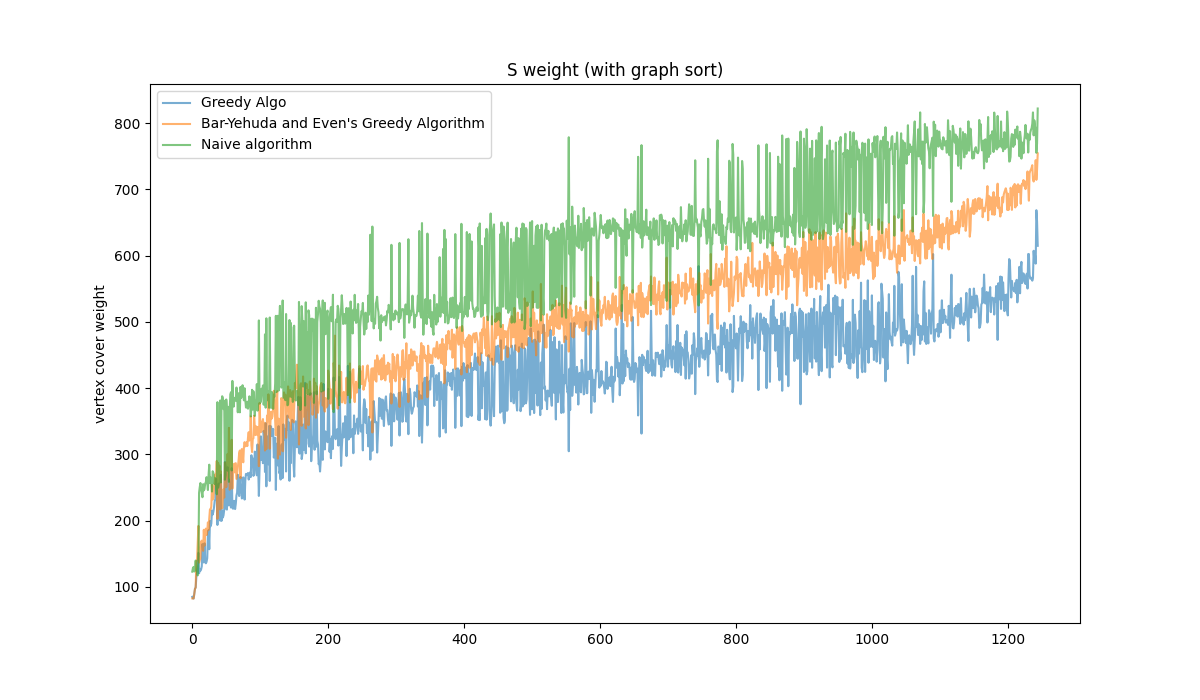
\includegraphics[scale=0.5]{img/simple_plot}
  \end{figure}
  Из графика видно, что в большинстве случаев алгоритм \ref{greedyAlgo} работает лучше других, 
  а наивный -- хуже. \\
  Для детального сравнения алгоритмов \ref{greedyAlgo} и \ref{bye_algo} будем считать отношение весов 
  ответов на одном и том же взвешенном графе и примерное распределение этой величины:
  \begin{figure}[H]
    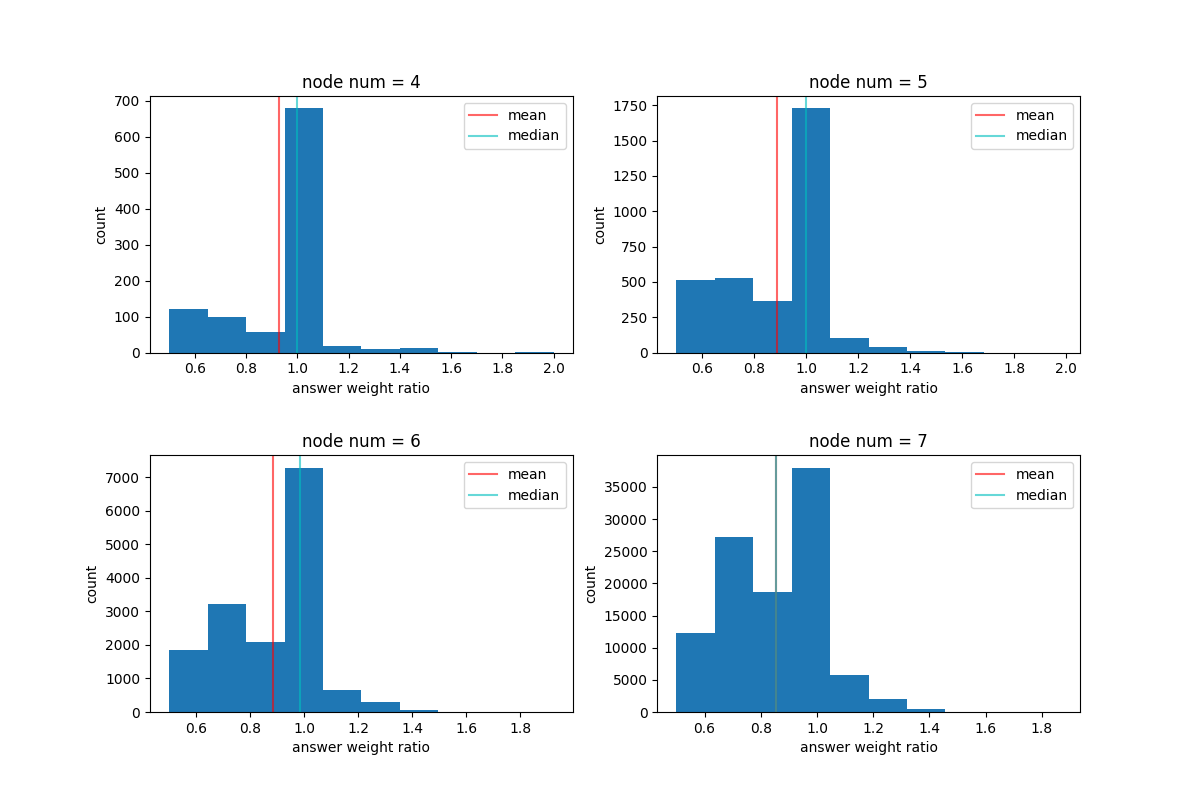
\includegraphics[scale=0.5]{img/simple_hists}
  \end{figure}
  Нетрудно заметить, что это отношение всегда находится между 0.5 и 2 
  (оба алгоритма дают 2-приближение минимального вершинного покрытия),
  а также, что в большинсве случаев (медиана) алгоритм \ref{greedyAlgo} дает лучший ответ, 
  чем \ref{bye_algo}.
  \subsection{Случайные графы $G(n, p)$}
  Тут построим большие случайные графы и проведем те же наблюдения, 
  а также посмотрим на время исполнения.
  \begin{figure}[H]
    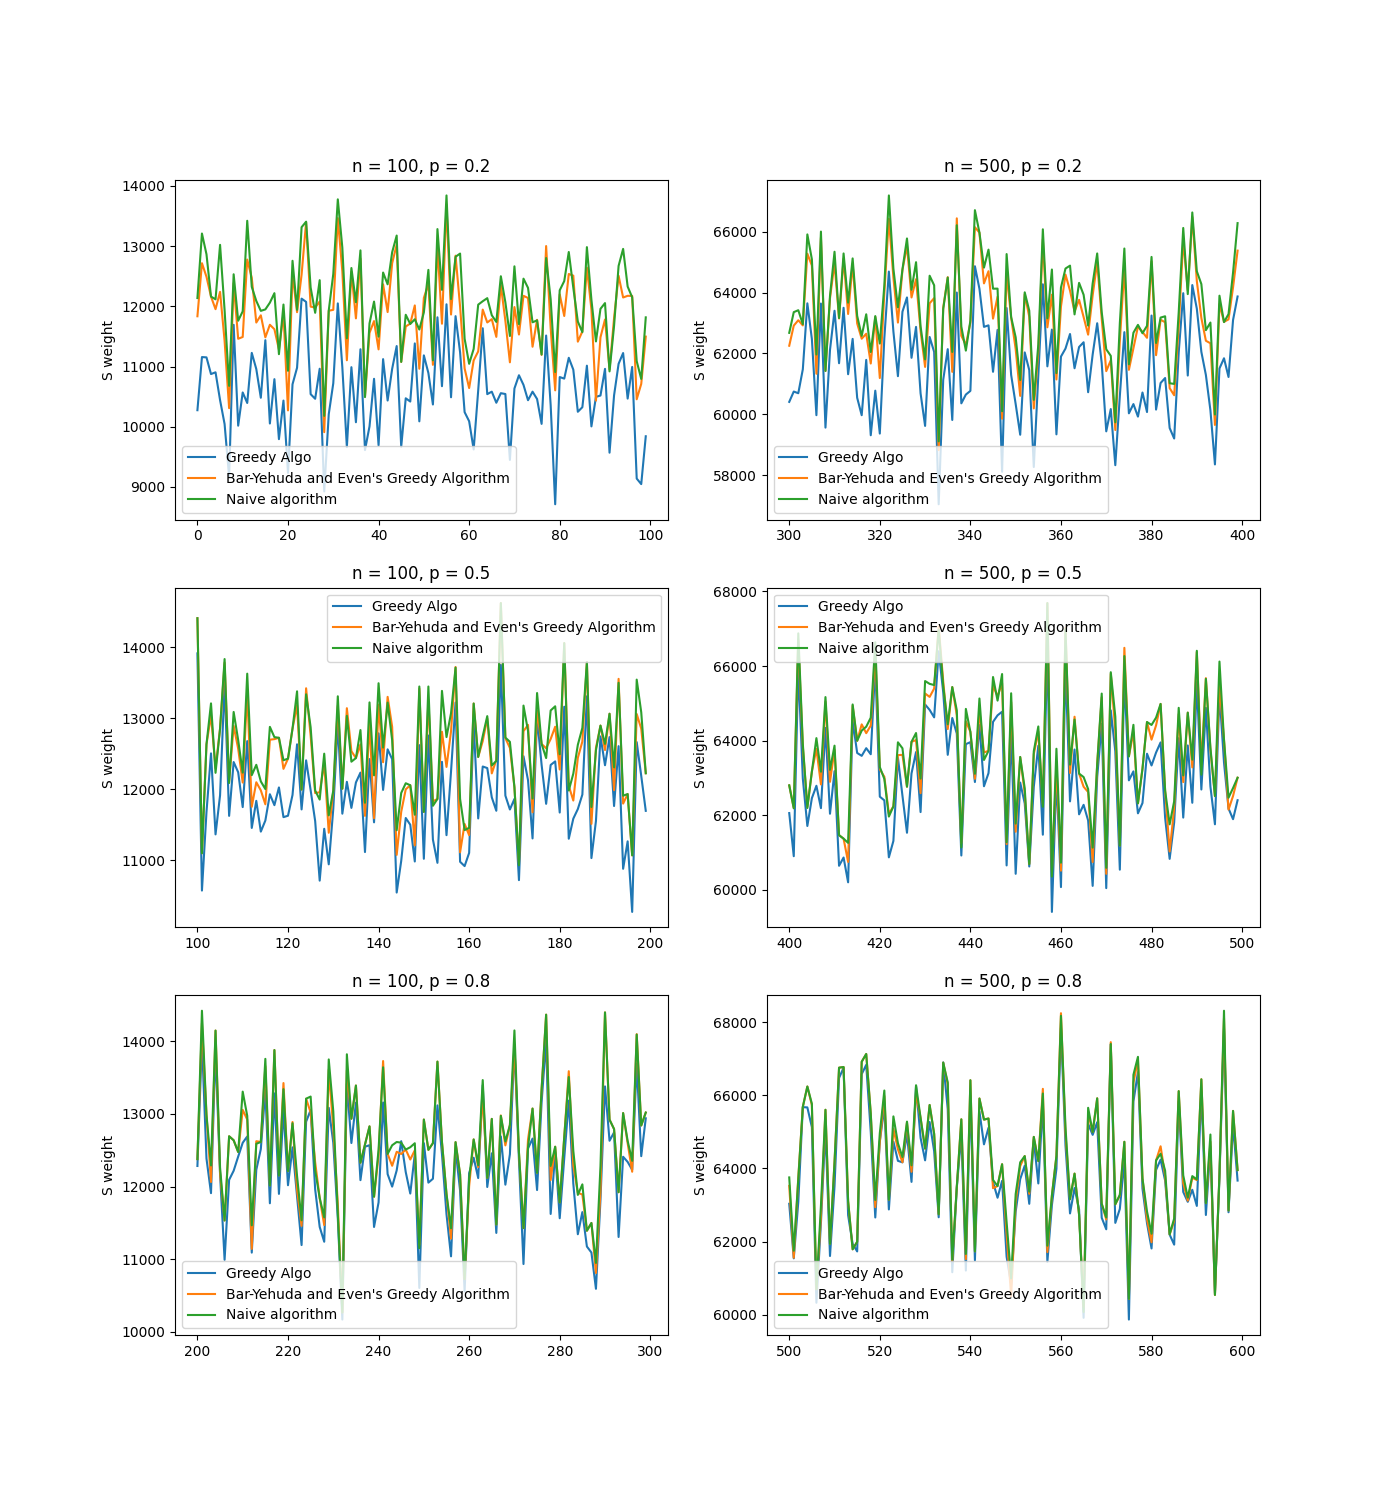
\includegraphics[scale=0.5]{img/gnp_plots}
  \end{figure}
  Тут можно отметить, что с увелиением плотности графа или 
  количества вершин алгоритмы начинают вести себя почти одинаково.
  Случай $n=500, p=0.8$ анализировать вообще бессмысленно.
  
  Давайте построим аналогичные графики по времени.
  \begin{figure}[H]
    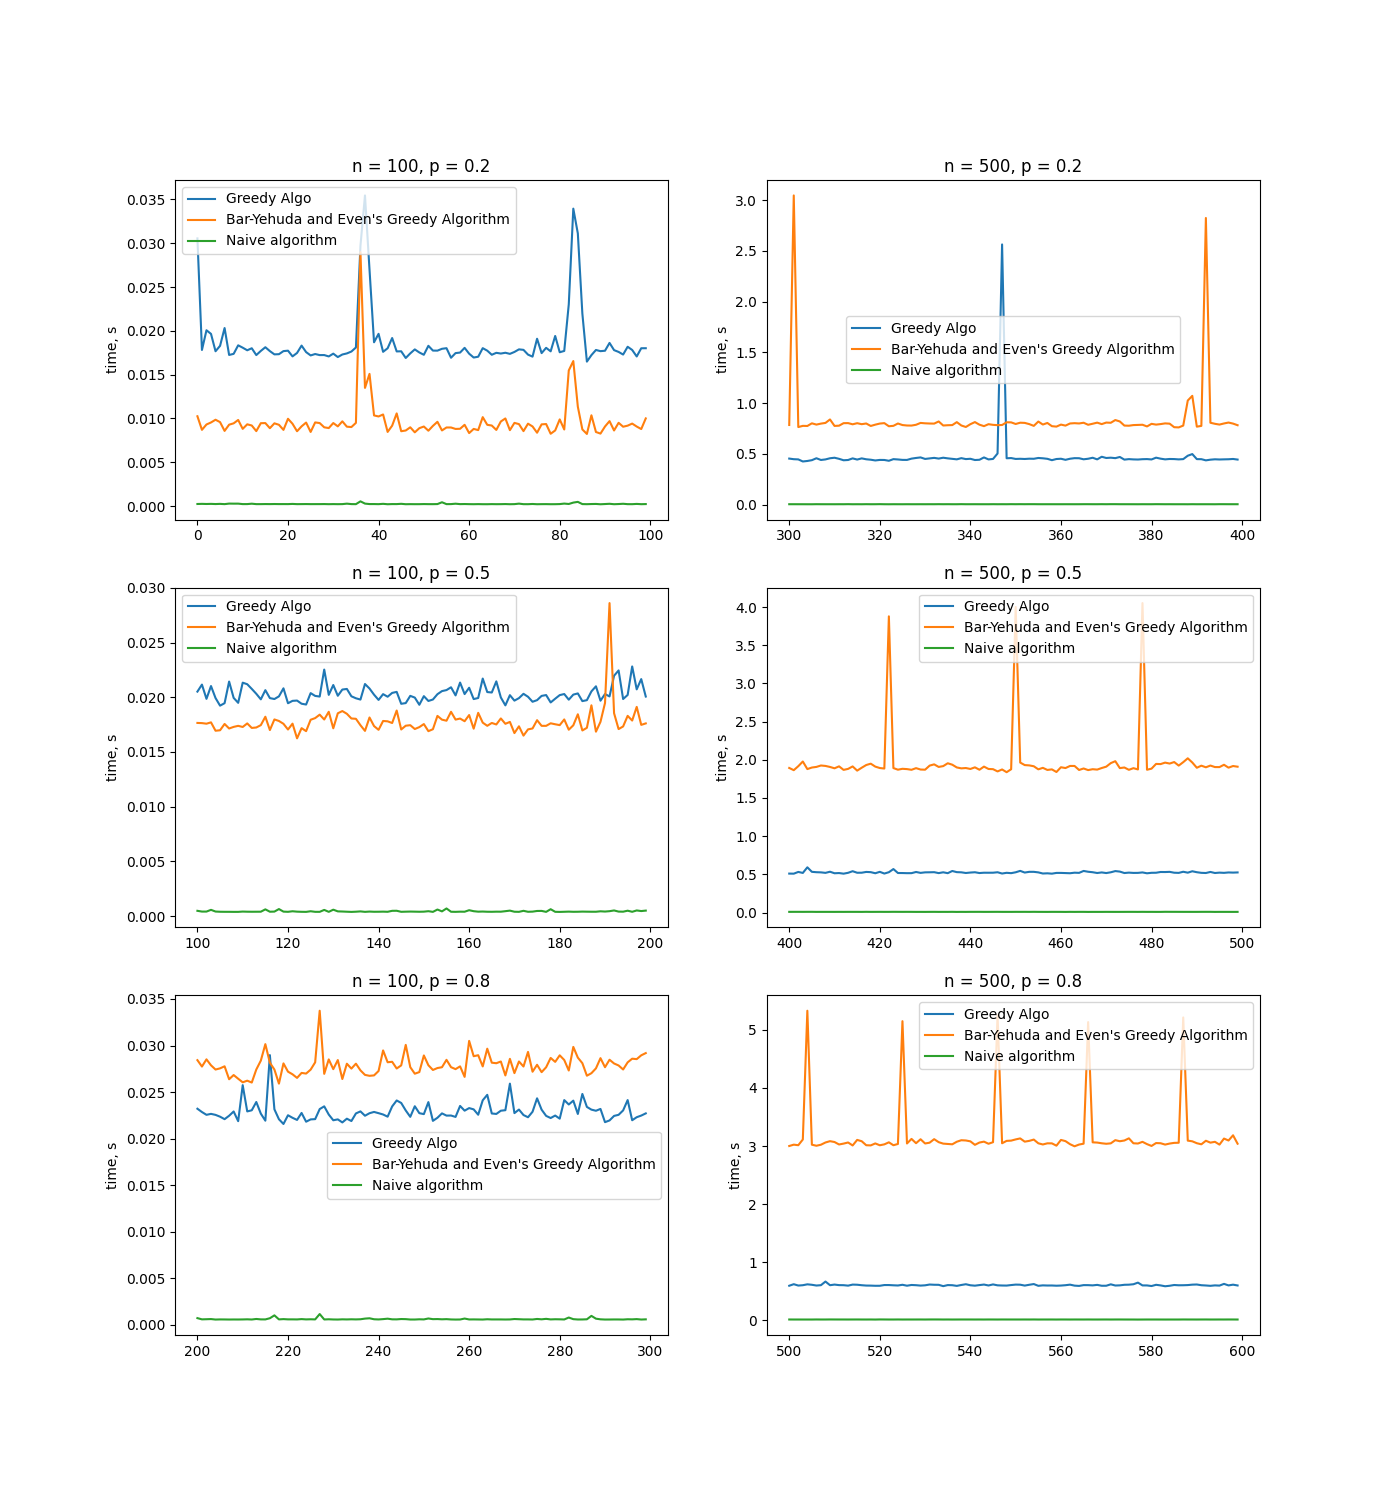
\includegraphics[scale=0.4]{img/gnp_time_plots}
  \end{figure}
  Видно, что наивный алгоритм всегда работает быстрее (неудивительно). 
  Между двумя другими алгоритмами разница несущественна, и может быть списана на реализацию.
  
  Выведем отношение весов ответов алгоритмов \ref{greedyAlgo} и \ref{bye_algo}
  \begin{figure}[H]
    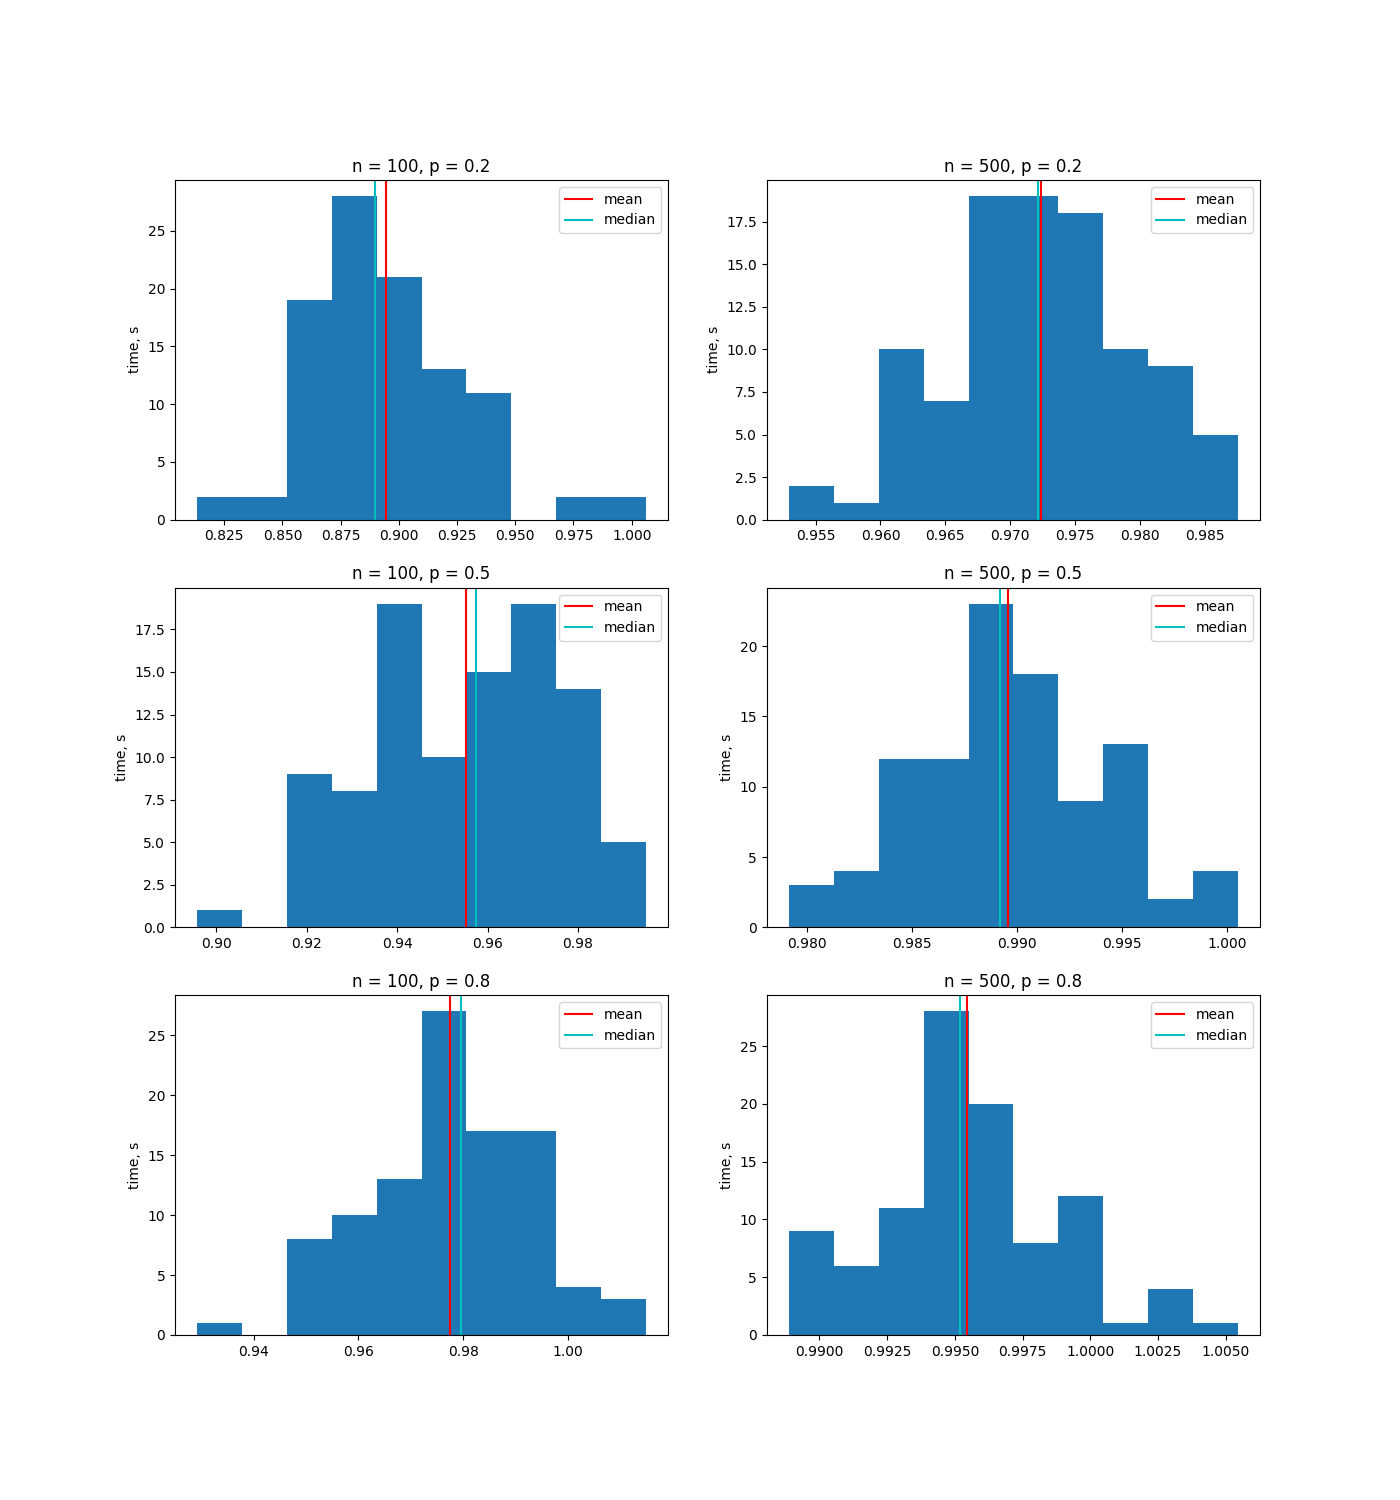
\includegraphics[scale=0.5]{img/gnp_ratio_hists}
  \end{figure}
  Тут статистика соответствует полученным ранее результатам. 
  А именно, при большой плотности ребер и количестве вершин, результаты алгоритмов очень близки.
  Однако алгоритм \ref{greedyAlgo} все же почти всегда немного лучше \ref{bye_algo}.
  \subsection{Другие виды графов}
  \subsubsection{Планарные}
  Данные были взяты с \cite{graphs_source}.
  \begin{figure}[H]
    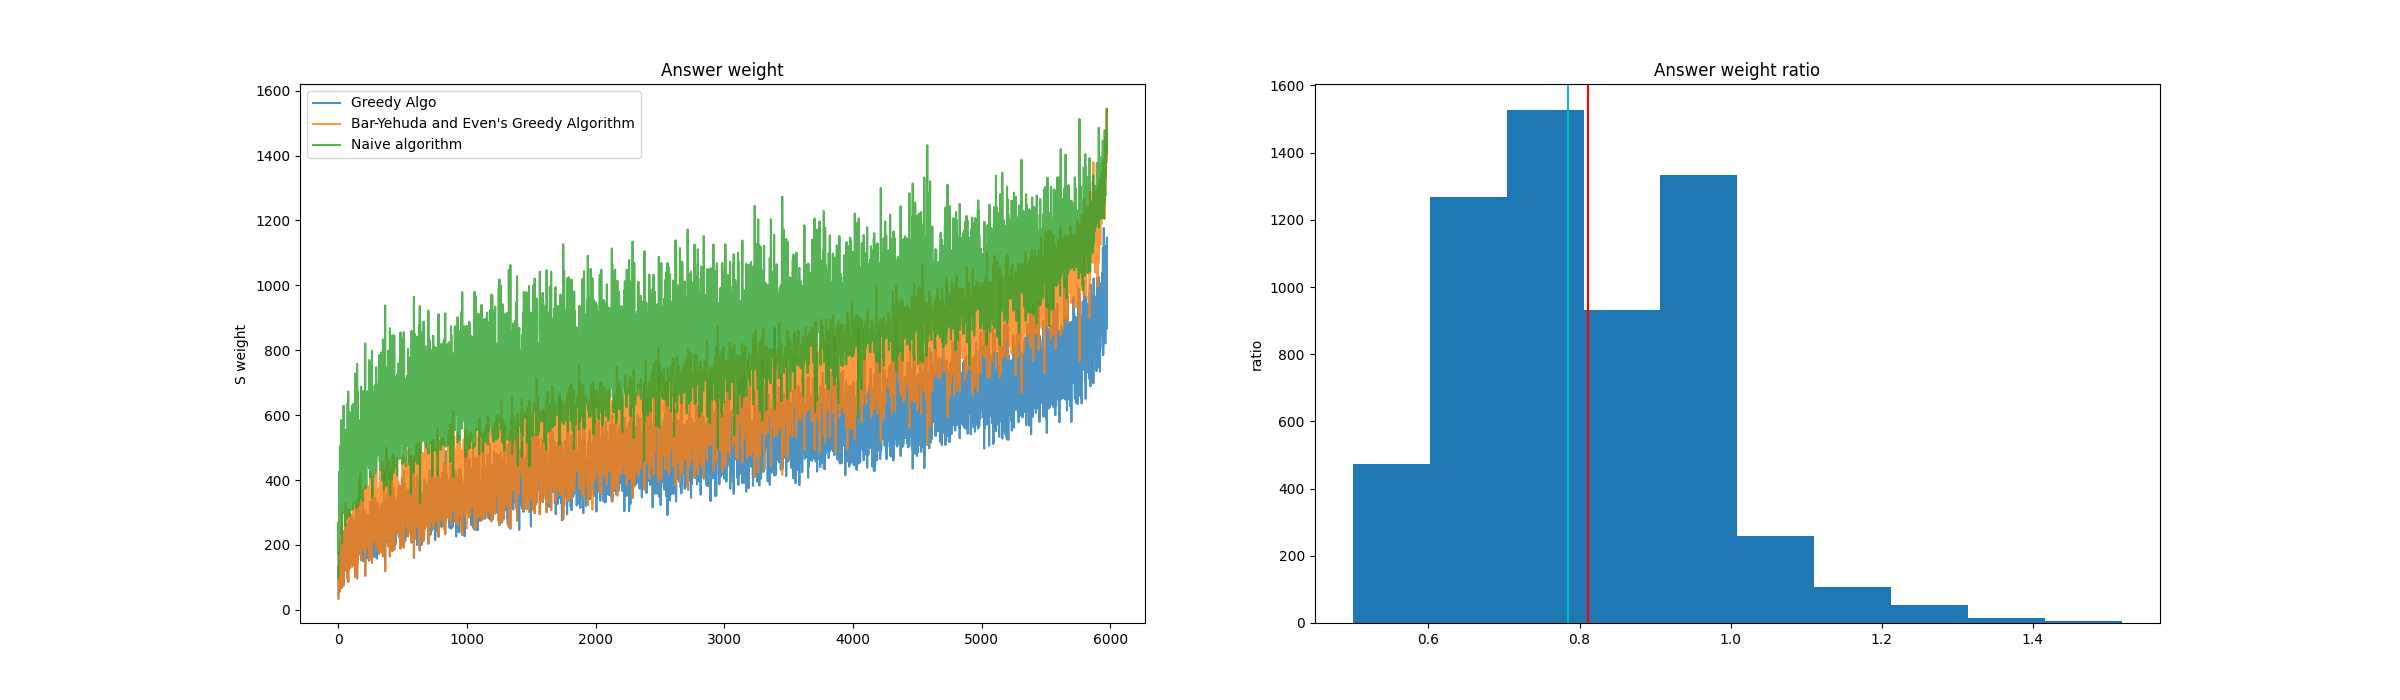
\includegraphics[scale=0.3]{img/planar8_quick}
  \end{figure}
  \subsubsection{Деревья}
  \begin{figure}[H]
    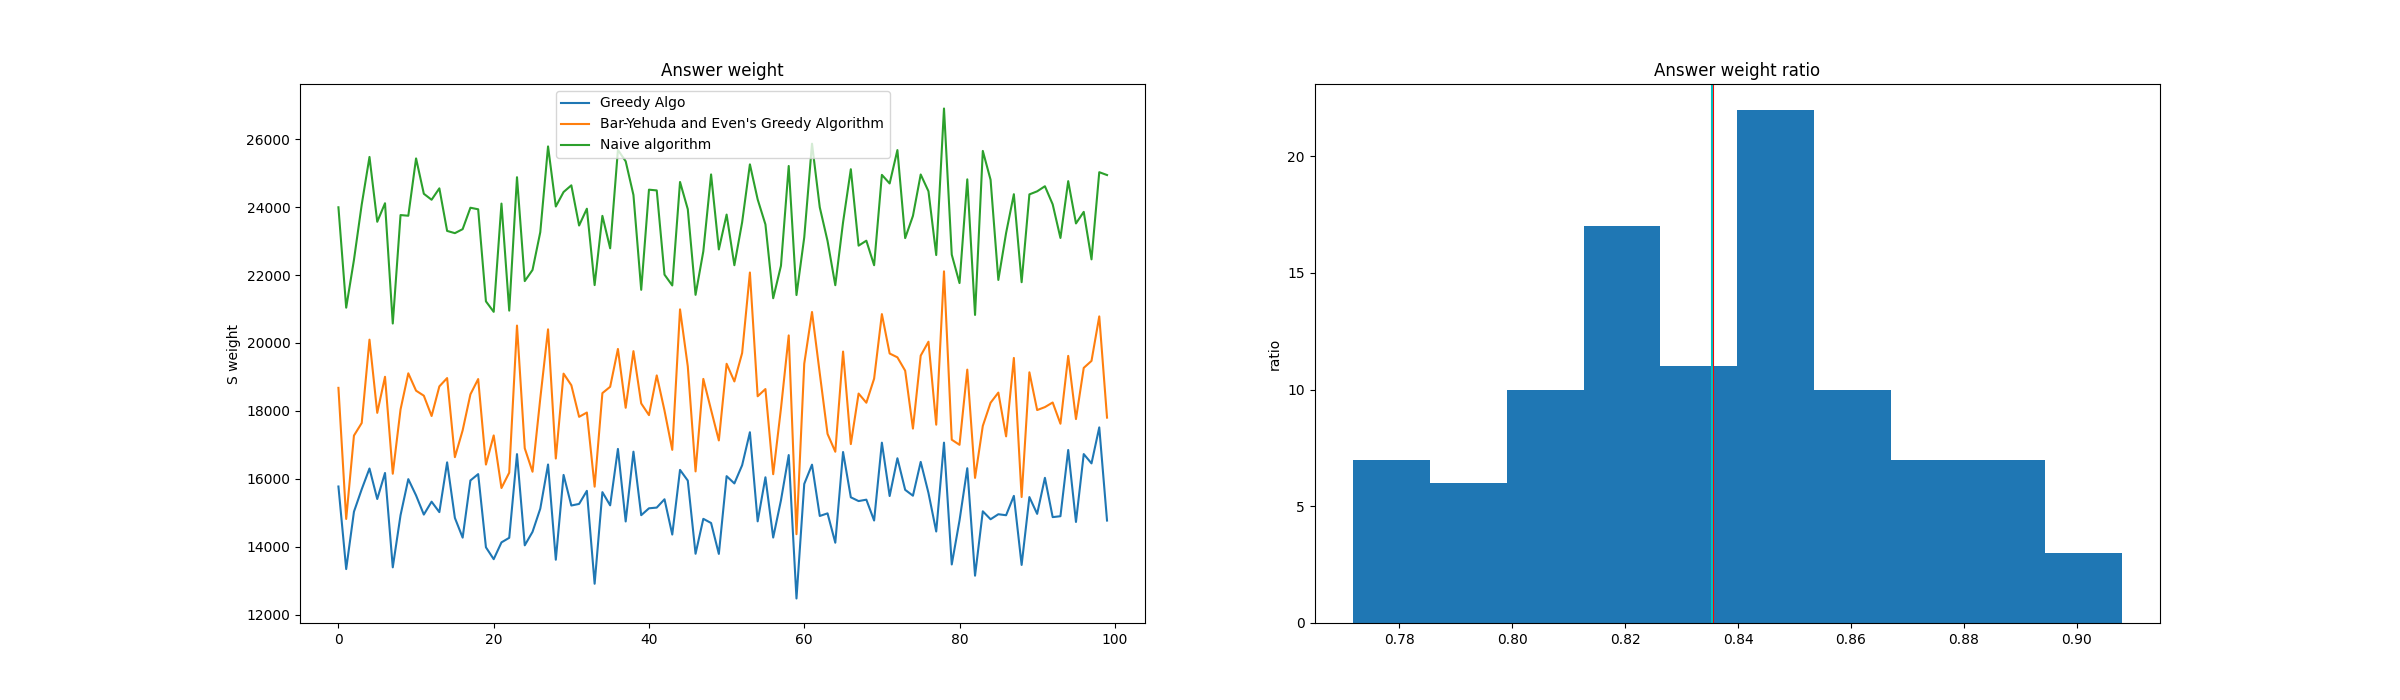
\includegraphics[scale=0.3]{img/random_tree_quick}
  \end{figure}
  \subsubsection{Сильно регулярные}
  Данные были взяты с \cite{graphs_source}.
  \begin{figure}[H]
    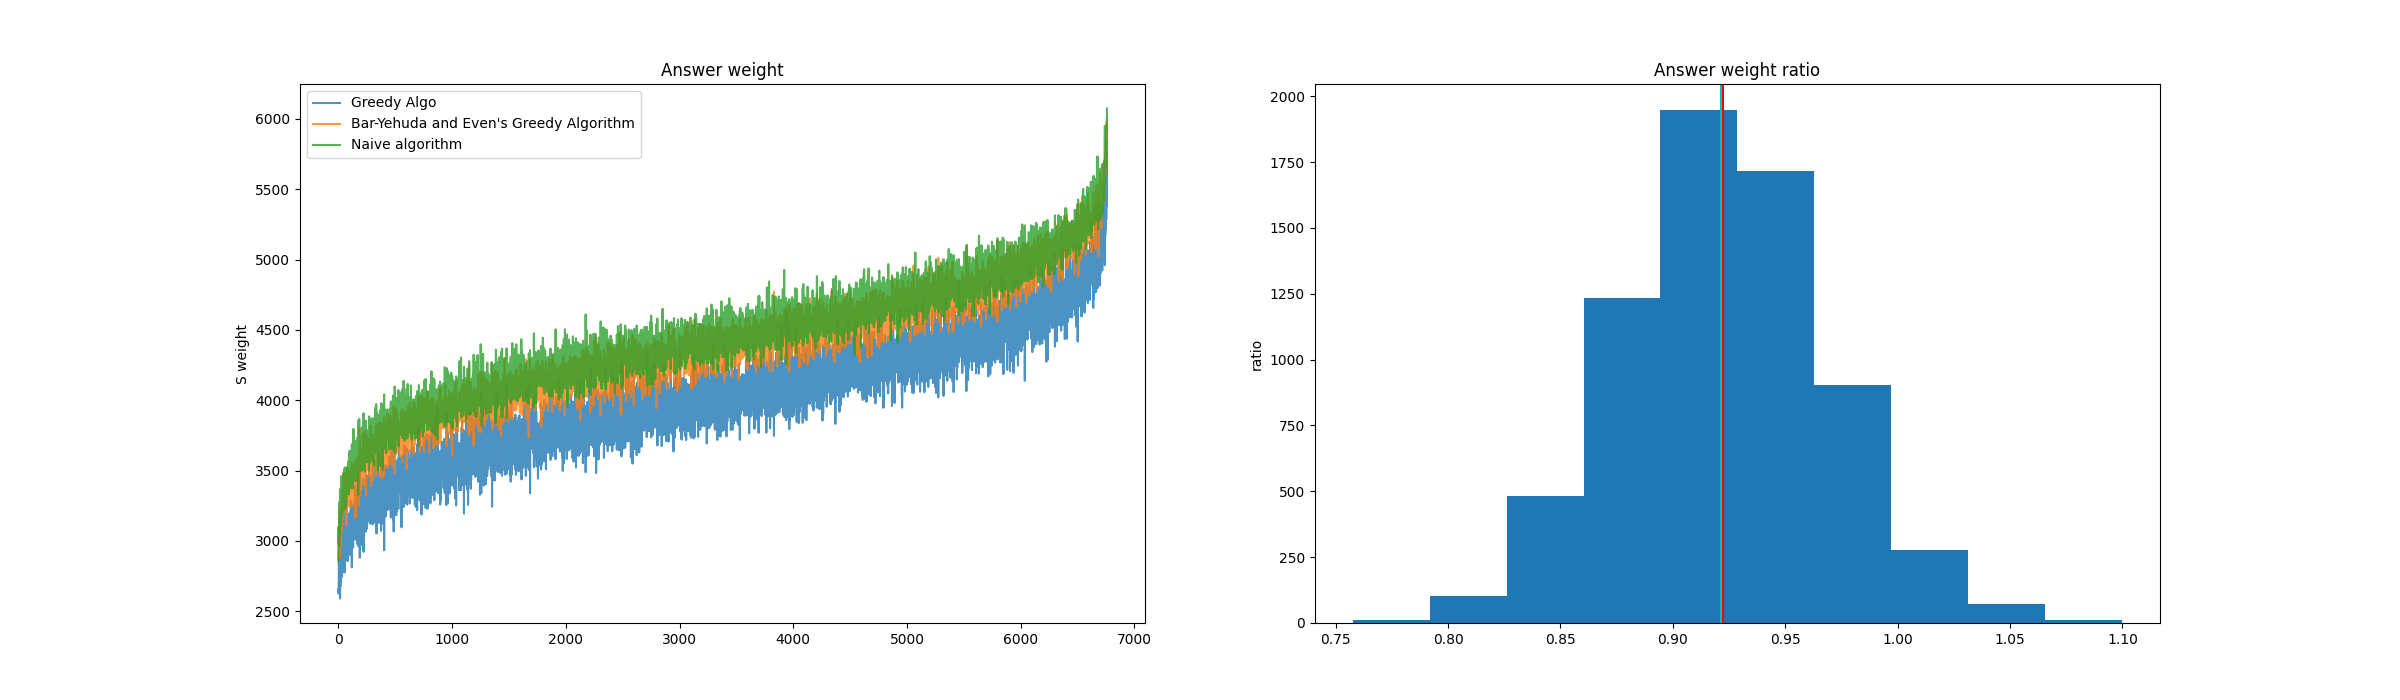
\includegraphics[scale=0.3]{img/srg_quick}
  \end{figure}
  Во всех трех случаях отмеченные закономерности также работают.
  \section{Выводы}
  Построенный алгоритм $2$-приближения является достаточно эффективным в среднем 
  даже в сравнении с другим алгоритмом $2$-приближения.
  \begin{thebibliography}{1}
    \bibitem{bye_algo_ref}
      Samir Khuller, Advanced Algorithms, Lectures 4 and 5. 
      (\url{https://www.cs.umd.edu/class/fall2018/cmsc858E/pdfs/651/vc.pdf})
    \bibitem{main_source}
      А.В.Кононов, П.А.Кононова, Приближенные алгоритмы для решения NP-Трудных задач,\\
      (\url{http://old.math.nsc.ru/LBRT/k5/Kononov/Kononovs_teaching_book.pdf})
    \bibitem{graphs_source}
      Примеры графов,
      (\url{http://users.cecs.anu.edu.au/~bdm/data/graphs.html})

  \end{thebibliography}
\end{document}